% ----------------------------------------------	
\pagestyle{plain}
\whitetext{\chapter{Introduction}}
\pagecolor{ccteal}
\fontfamily{phv}
%\vspace*{\stretch{.5}}
\pagebreak
\newpagecolor{white}
\pagestyle{fancy}
\fancyhf{}
\renewcommand{\chaptermark}[1]{\markboth{#1}{}}
\fancyfoot[LE,RO]{\thepage}

	\begin{minipage}[t][.5\textheight][t]{\textwidth}
	\textcolor{ccteal}{\section{Overview}}
	
	\input{\rootpath/TEXT/overview_text/\tds_overview}
	
	\end{minipage}
\begin{minipage}[c][.39\textheight][c]{\textwidth}
\begin{table}[H]
\small

\input{\rootpath/TABLES/overview_table/\tds_overview_table}
\end{table}

\begin{centering}
\input{\rootpath/TABLES/typology_table/\tds_typology}
\end{centering}
\end{minipage}
\pagebreak

\newgeometry{left=0in, right=0in, top=0in, bottom=0in}
\fakesection{Context Map}
\afterpage{%
    \clearpage% flush all other floats
    \ifodd\value{page}
    %\else% uncomment this else to get odd/even instead of even/odd
        \expandafter\afterpage% put it on the next page if this one is odd
    \fi
    {%
    \begin{figure}[H]
    	\raggedleft
        \includegraphics[height=11in]{\rootpath/MAPS/context_maps/\tds_context_1.png}%
    \end{figure}
    \clearpage
    \begin{figure}[H]
    	\raggedright
        \includegraphics[height=11in]{\rootpath/MAPS/context_maps/\tds_context_2.png}%
    \end{figure}
    \clearpage
    }%
}
\restoregeometry
\pagebreak
%-------------------------------------------
\pagestyle{plain}
\whitetext{\chapter{Waste Services and Assets}}
\pagecolor{ccorange}
\pagebreak
\newpagecolor{white}
\pagestyle{fancy}
\fancyhf{}
\renewcommand{\chaptermark}[1]{\markboth{#1}{}}
\fancyfoot[LE,RO]{\thepage}

\textcolor{ccorange}{\section{Waste Distribution}}
%%%% TO-DO: AUTOMATE TEXT GENERATION %%%
The goal of the waste calculator is to understand the amount of waste generated at each development and consolidation. This knowledge is imperative to interpreting what assets are necessary in order for each consolidation to run most efficiently. Sumner consolidation is not serviced by DSNY daily. Once the compactors are full, DSNY is called to pick it up. The Sumner Consolidation has (4) 30-CY external compactors and containers, totaling 766.36 ft2 of storage space for waste. Given the rate at which waste is produced at NYCHA properties, these containers will fill up in about (3) days at the Sumner Consolidation. The average weight of the containers at capacity should be about (3) tons.

\begin{table}[H]
\begin{threeparttable}
\small

\input{\rootpath/TABLES/waste_distribution_table/\tds_wd_table}

\begin{tablenotes}
\item [1] Assumes 5lbs of waste is produced daily in each unit.
\item [2] Includes miscellaneous garbage as well as uncaptured recyclables, organics, e-waste, and textiles.
\item [3] Primary method of trash collection, via chute. Assumes a 75\% capture rate.
\item [4] Secondary method of trash collection. Assumes a 25\% capture rate
\item [5] Capture rates of recyclables at NYCHA portfolio-wide: 30\% of MGP, 50\% of Cardboard, and 20\% of Paper. 
%\item[5] Organics, e-waste, and textiles have a capture rate of 0\%.
\end{tablenotes}
\end{threeparttable}
\end{table}
\pagebreak

\textcolor{ccorange}{\section{Waste Services and Assets}}
%%% TO-DO: AUTOMATE TEXT GENERATION %%%
DSNY does not provide curbside collection at this site. Caretakers are responsible for collecting all
waste throughout the consolidation and bringing it to the external compactors. All bulk is left outside the
buildings for collection to the 30-yard bulk container located at 303 Vernon. Household waste produced
in Sumner goes to one of the three waste yards on site. Household waste produced at
Bedford-Stuyvesant Rehab is brought to the curb for pick up by the caretakers using a Ford pick-up
truck and driven to the waste yards at either Sumner or 303 Vernon.
\begin{table}[H]
\small
%%% TO-DO: AUTOMATE WASTE SERVICES AND ASSETS TABLE %%%
\begin{tabular}{V{1.5in}|V{1.5in}|V{1.5in}|V{1.5in}|}
\cline{2-4}
                                                                                   & \cellcolor{ccorange}{\color[HTML]{FFFFFF} 303 Vernon Avenue} & \cellcolor{ccorange}{\color[HTML]{FFFFFF} Bedford-Stuyvesant Rehab} & \cellcolor{ccorange}{\color[HTML]{FFFFFF} Sumner Houses} \\ \hline
\multicolumn{1}{|V{1.5in}|}{\cellcolor{ccorangelight}Household Waste (DSNY)}               & 1 Waste Yard; 1 Hydraulic Exterior Compactor                     & Transfer to 303 Vernon or Sumner                                        & 2  Waste Yards with 1 Hydraulic Exterior Compactor Each      \\ \hline
\multicolumn{1}{|V{1.5in}|}{\cellcolor{ccorangelight}Bulk Waste}                           & IESI with One(?) 30-Yard Container                               & Transfer to 303 Vernon                                                  & Transfer to 303 Vernon                                       \\ \hline
\multicolumn{1}{|V{1.5in}|}{\cellcolor{ccorangelight}Recycling: Paper and Cardboard}       & TK                                                               & TK                                                                      & TK                                                           \\ \hline
\multicolumn{1}{|V{1.5in}|}{\cellcolor{ccorangelight}Recycling: Metal, Glass, and Plastic} & DSNY Curb Setout                                                 & DSNY Curb Setout                                                        & DSNY Curb Setout                                             \\ \hline
\multicolumn{1}{|V{1.5in}|}{\cellcolor{ccorangelight}Recycling: Mattresses}                & N/A                                                              & N/A                                                                     & TK                                                           \\ \hline
\multicolumn{1}{|V{1.5in}|}{\cellcolor{ccorangelight}Recycling: Textiles}                  & N/A                                                              & N/A                                                                     & TK                                                           \\ \hline
\multicolumn{1}{|V{1.5in}|}{\cellcolor{ccorangelight}Recycling: E-Waste}                   & N/A                                                              & N/A                                                                     & TK                                                           \\ \hline
\end{tabular}
\end{table}
\pagebreak

\textcolor{ccorange}{WASTE ASSET MAP}
\begin{figure}[H]
\raggedright
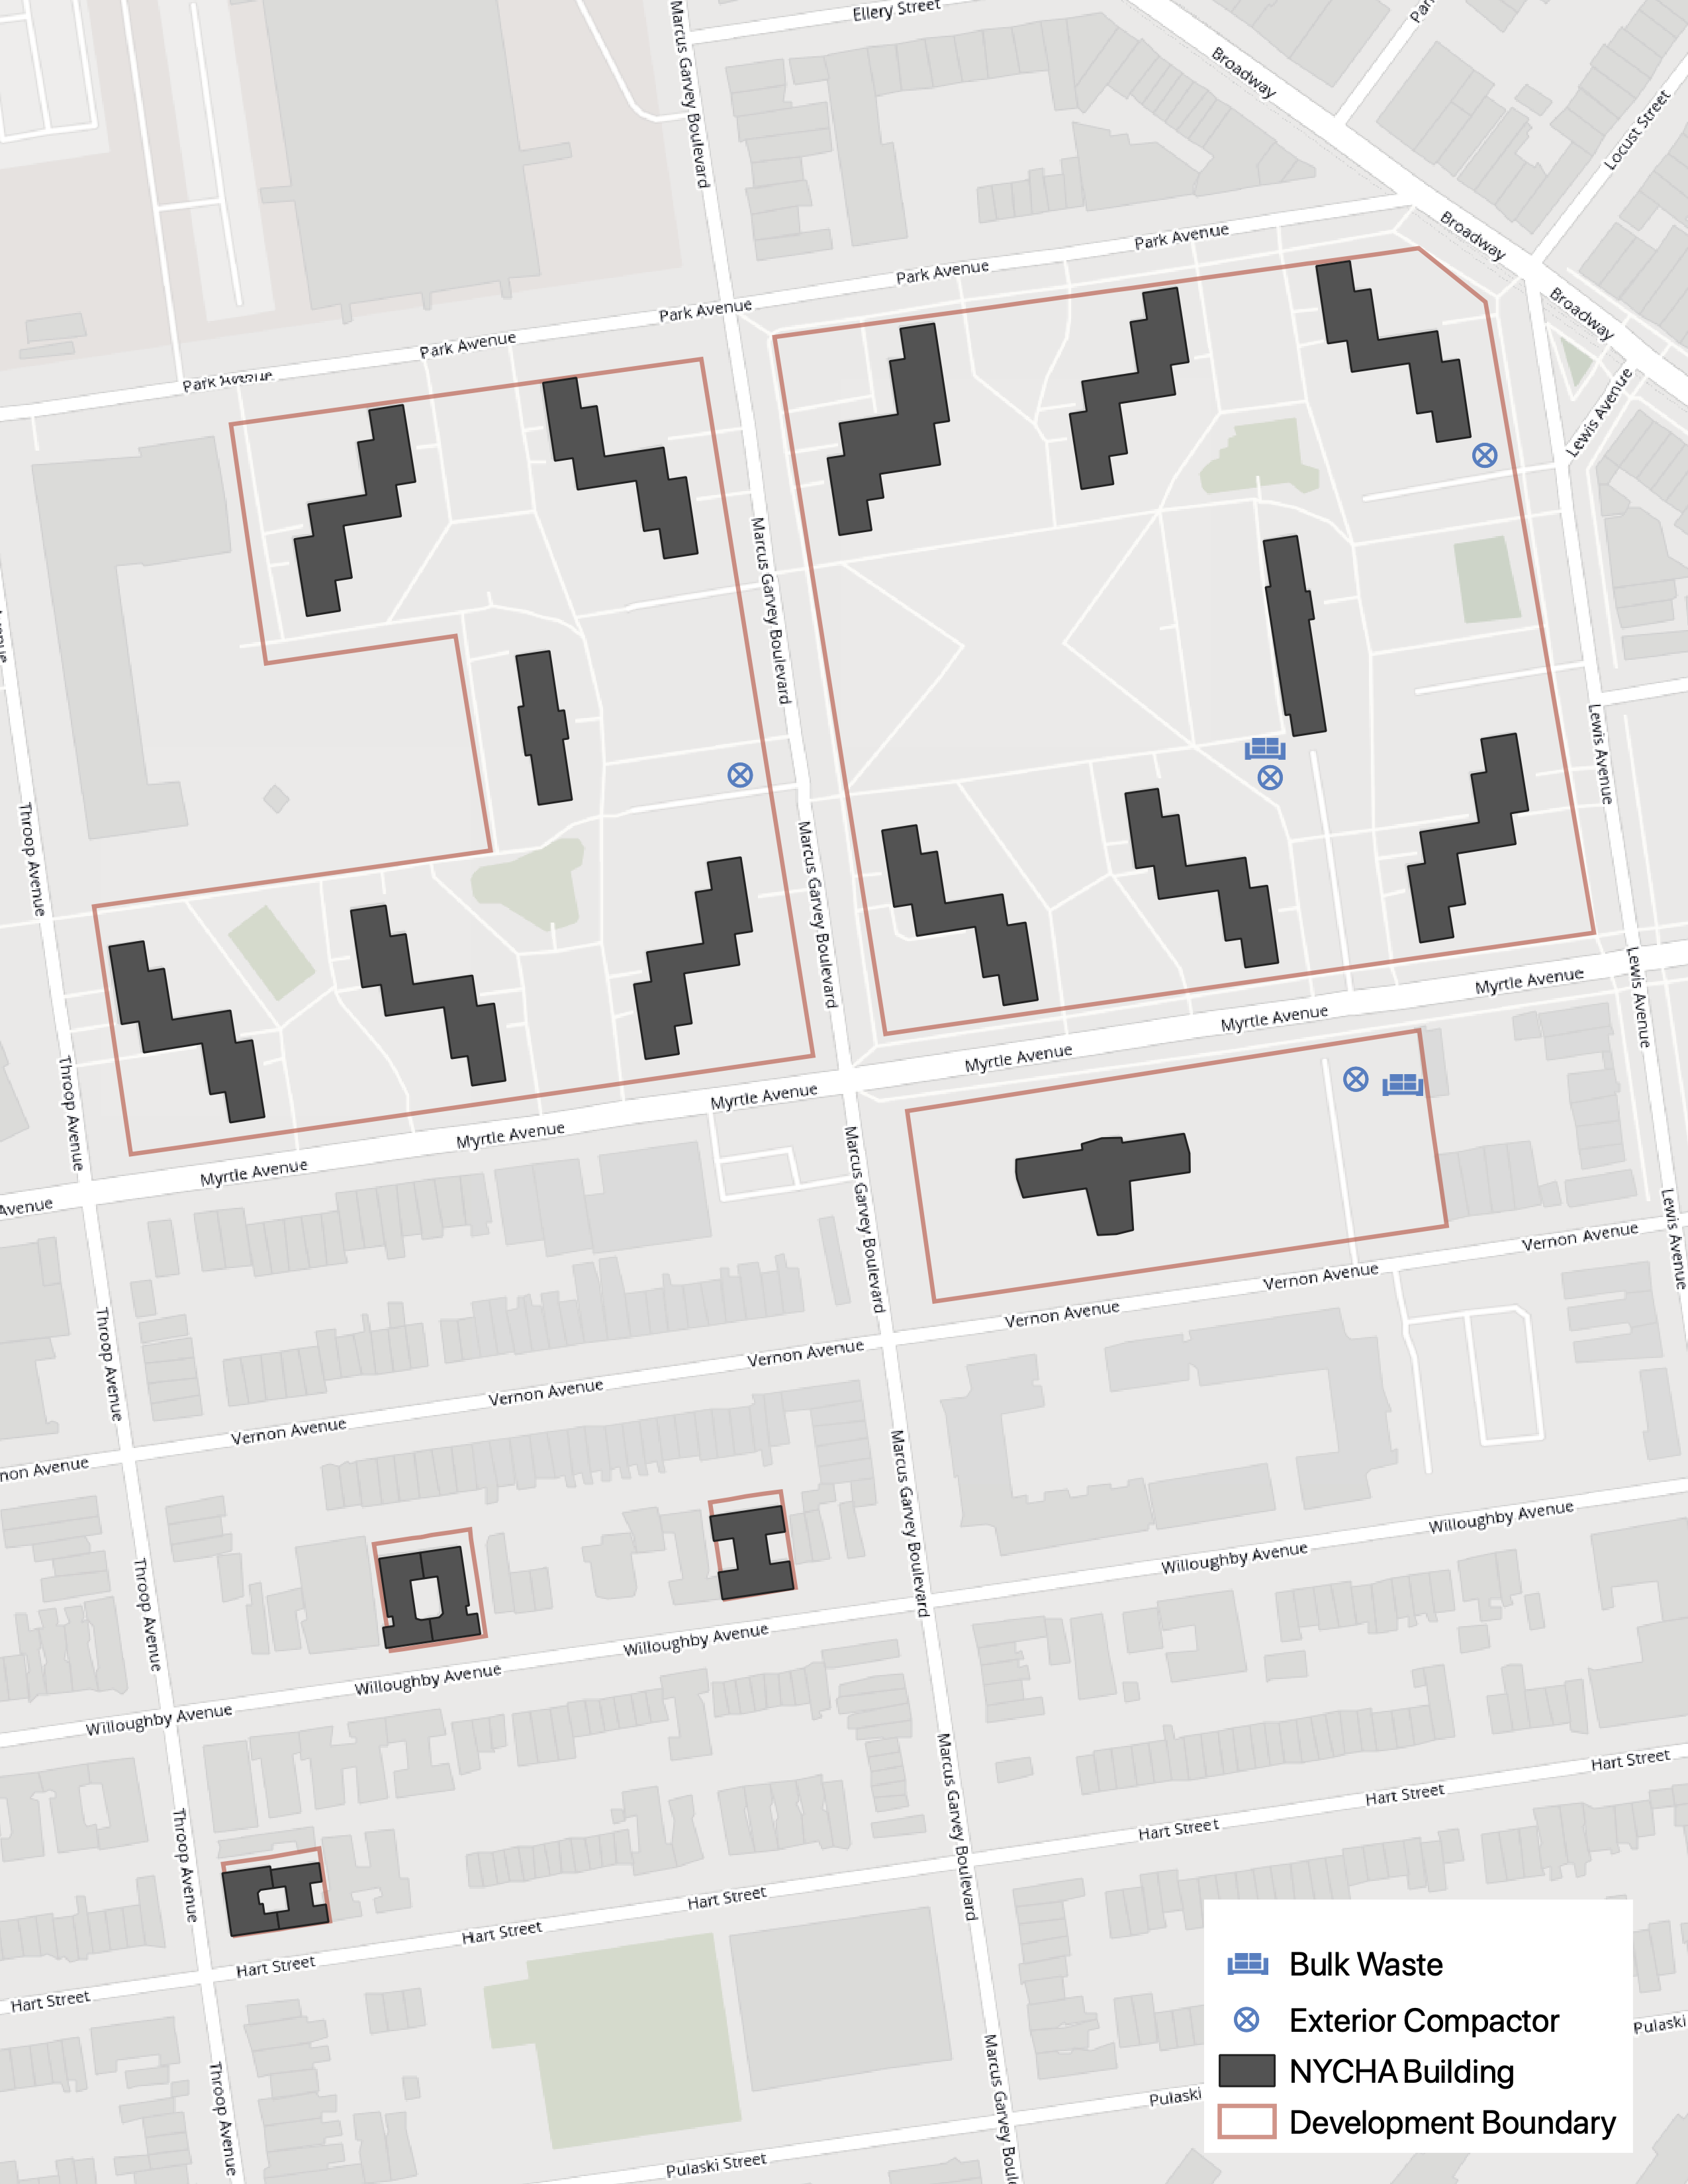
\includegraphics[width=.95\textwidth]{\rootpath/MAPS/asset_maps/073_asset_map.png}
\end{figure}
\pagebreak

\textcolor{ccorange}{WASTE ASSETS}

\begin{table}[H]
\small
%%% TO-DO: AUTOMATE WASTE ASSETS TABLE %%%
\begin{tabular}{V{.25\columnwidth}|V{.15\columnwidth}|V{.15\columnwidth}|V{.25\columnwidth}|V{.15\columnwidth}|}
\cline{2-5}
                                                                                              & \cellcolor{ccorangelight}{\color[HTML]{000000} Internal Compactors} & \cellcolor{ccorangelight}{\color[HTML]{000000} External Compactors} & \cellcolor{ccorangelight}{\color[HTML]{000000} Other External Assets}   & \cellcolor{ccorangelight}{\color[HTML]{000000} Recycling Bins} \\ \hline
\multicolumn{1}{|V{.25\columnwidth}|}{\cellcolor{ccorange}{\color[HTML]{FFFFFF} 303 Vernon Avenue}}        & 1; last replaced TK                                                & 1                                                                  & Bulk crusher, cardboard baler, mattress recycling, electric tilt truck & TK                                                            \\ \hline
\multicolumn{1}{|V{.25\columnwidth}|}{\cellcolor{ccorange}{\color[HTML]{FFFFFF} Bedford-Stuyvesant Rehab}} & 5; last replaced TK                                                & 0                                                                  & Bulk crusher, cardboard baler, mattress recycling, electric tilt truck & TK                                                            \\ \hline
\multicolumn{1}{|V{.25\columnwidth}|}{\cellcolor{ccorange}{\color[HTML]{FFFFFF} Sumner Houses}}            & 24; last replaced TK                                               & 3                                                                  & Bulk crusher, cardboard baler, mattress recycling, electric tilt truck & TK                                                            \\ \hline
\end{tabular}
\end{table}

\textcolor{ccorange}{SUMNER CONSOLIDATION ASSETS}
\begin{table}[H]
\begin{tabular}{m{.33\columnwidth}m{.33\columnwidth}m{.33\columnwidth}}
{\color{ccorange} X Trucks} & {\color{ccorange} X Bobcats} & {\color{ccorange} X Other} \\

\includegraphics[width=.25\columnwidth]{\rootpath/IMAGES/truck.png}                            & 
\includegraphics[width=.25\columnwidth]{\rootpath/IMAGES/bobcat.png}                             & 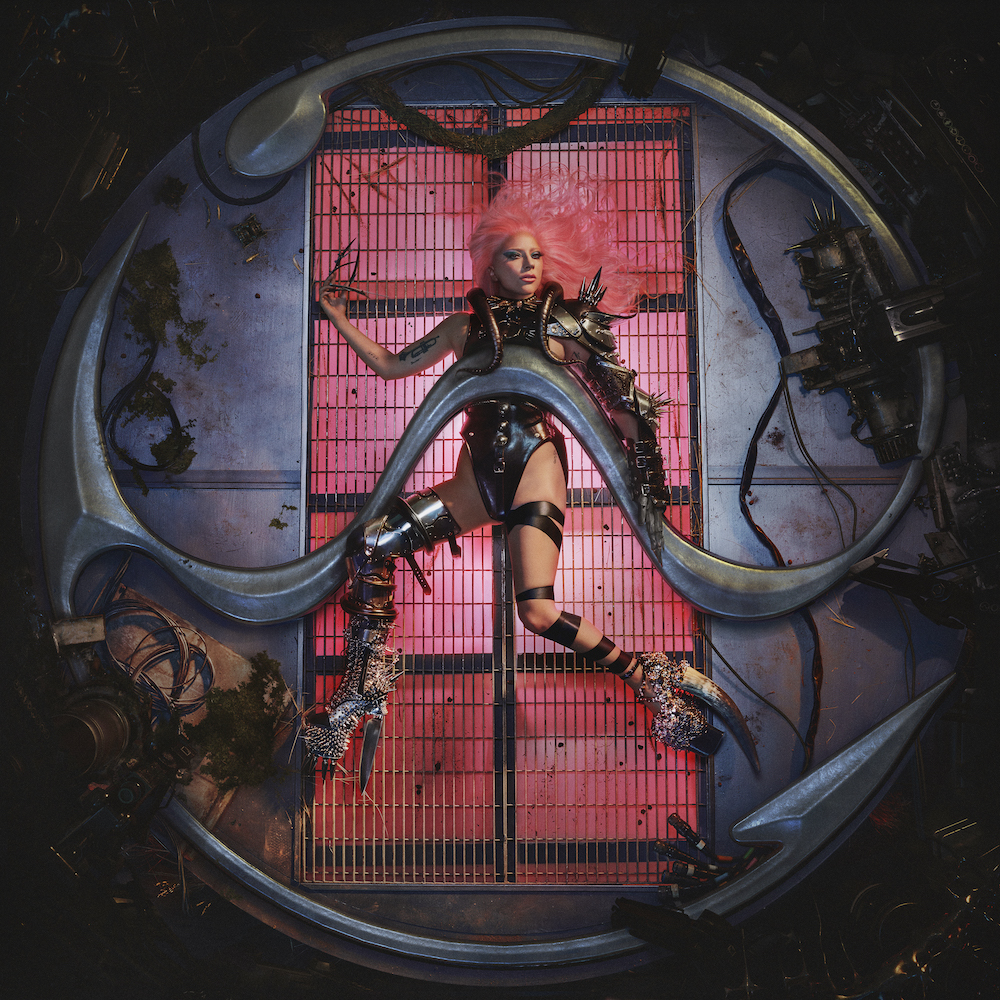
\includegraphics[width=.25\columnwidth]{\rootpath/IMAGES/chromatica.jpg}                          
\end{tabular}
\end{table}
\pagebreak
\textcolor{ccorange}{\section{Capital Improvements}}

\begin{table}[H]

\input{\rootpath/TABLES/capital_projects_table/\tds_capital_projects}

\end{table}
\pagebreak

\textcolor{ccorange}{PRIORITIES}

PLACEHOLDER TEXT AND TABLES AND SUCH TO FIGURE OUT PAGE COLOR SETTINGS -- WILL FILL IN LATER, ONCE PRELIMINARY ANALYSIS IS COMPLETE
\pagebreak
%-------------------------------------------
\pagestyle{plain}
\whitetext{\Chapter{Staffing}}
\pagecolor{ccfuschia}
\pagebreak
\newpagecolor{white}
\pagestyle{fancy}
\fancyhf{}
\renewcommand{\chaptermark}[1]{\markboth{#1}{}}
\fancyfoot[LE,RO]{\thepage}


\textcolor{ccfuschia}{STAFFING STRUCTURE}
\begin{figure}[H]
	\resizebox{\textwidth}{!}{
	\centering
	\begin{tikzpicture}[node distance=3cm]
	\node (vp) [processwide] {VP of Operations};
	\node (borodr) [processwide, below of=vp] {Borough Director};
	\node(ram) [processwide, below of=borodr] {Regional Asset Manager};
	\node (pm) [processwide, below of=ram] {Property Manager};
	\node (super) [process, below of=pm, xshift=-5cm] {Superintendent};
	\node (asuper) [process, below of=super] {Assistant Superintendent};
		\node (mtn) [process, below of=asuper, xshift=-3.5cm] {Maintenance Workers};
		\node (spc) [process, below of=asuper] {Supervisor of Caretakers};
			\node (crt) [process, below of=spc] {Caretakers\\(X and J)};
		\node (spg) [process, below of=asuper, xshift=3.5cm] {Supervisor of Grounds};
			\node (crtg) [process, below of = spg] {Caretakers (G)};			
		
	\node (apm)[process, below of=pm, xshift=5cm] {Assistant Property Manager};
		\node (sec) [process, below of=apm, xshift = -2.5cm] {Secretaries};
		\node (asst) [process, below of=apm, xshift = 2.5cm] {Housing Assistants};

	%\node (sub1) [subprocess, below of=pro1] {\nodepart{two} Subprogram};
	%\node (dec1) [decision, below of=sub1, yshift=-1cm] {Decision};
	%\node (com1) [comment, below of=dec1, xshift=-4cm, yshift=-1cm] {STEP 2};
	%\node (stop) [startstop, below of=dec1, yshift=-1cm] {Stop};

	%\draw [arrow] (dec1.west) -- ++(-1,0) node[anchor=south,pos=0.5] {No} |- (sub1.west);
	%\draw [arrow] (dec1) -- node[anchor=west] {Yes} (stop);

	\draw [arrow] (vp) -- (borodr);
	\draw [arrow] (borodr) -- (ram);
	\draw [arrow] (ram) -- (pm);
	\draw [arrow] (pm) -- (super);
	\draw [arrow] (super) -- (asuper);
		\draw [arrow] (asuper) -- (mtn);
		\draw [arrow] (asuper) -- (spc);
			\draw [arrow] (spc) -- (crt);
		\draw [arrow] (asuper) -- (spg);
			\draw [arrow] (spg) -- (crtg);
	
	\draw [arrow] (pm) -- (apm);
		\draw [arrow] (apm) -- (sec);
		\draw [arrow] (apm) -- (asst);
	\end{tikzpicture}
	}
\end{figure}

\pagebreak
\textcolor{ccfuschia}{ALLOCATED STAFF}

\begin{table}[H]
\begin{threeparttable}


        \begin{tabular}{l|c|c|c|}
        \cline{2-4}
                                                                                     & \cellcolor{ccfuschia}{\color[HTML]{FFFFFF} Formula Allocation} & \cellcolor{ccfuschia}{\color[HTML]{FFFFFF} Budgeted} & \cellcolor{ccfuschia}{\color[HTML]{FFFFFF} Actual} \\ \hline
        \multicolumn{1}{|l|}{\cellcolor{ccfuschialight}Employees}                      & 45                                                      & 46                                                                & 41                                                        \\ \hline
        \multicolumn{1}{|l|}{\cellcolor{ccfuschialight}Property Manager}               & 1                                                      & 1                                                                & 1                                                       \\ \hline
        \multicolumn{1}{|l|}{\cellcolor{ccfuschialight}Asst. Property Manager}         & 1                                                      & 1                                                                & 1                                                       \\ \hline
        \multicolumn{1}{|l|}{\cellcolor{ccfuschialight}Secretaries}                    & 2                                                      & 2                                                                & 2                                                      \\ \hline
        \multicolumn{1}{|l|}{\cellcolor{ccfuschialight}Housing Assistants}             & 4                                                      & 4                                                                & 4                                                      \\ \hline
        \multicolumn{1}{|l|}{\cellcolor{ccfuschialight}Superintendent}                 & 1                                                      & 1                                                                & 1                                                      \\ \hline
        \multicolumn{1}{|l|}{\cellcolor{ccfuschialight}Assistant Superintendent}       & 2                                                      & 2                                                                & 2                                                      \\ \hline
        \multicolumn{1}{|l|}{\cellcolor{ccfuschialight}Supervisor of Caretakers (SOC)} & 1                                                      & 1                                                                & 1                                                      \\ \hline
        \multicolumn{1}{|l|}{\cellcolor{ccfuschialight}Supervisor of Grounds (SOG)}    & 1                                                      & 1                                                                & 1                                                      \\ \hline
        \multicolumn{1}{|l|}{\cellcolor{ccfuschialight}Maintenance Workers}            & 6                                                      & 6                                                                & 3                                                       \\ \hline
        \multicolumn{1}{|l|}{\cellcolor{ccfuschialight}Caretakers X}                   & 5                                                      & 5                                                                &                                                       \\ \cline{1-3}
        \multicolumn{1}{|l|}{\cellcolor{ccfuschialight}Caretakers J\tnote{1}}                   &                                                       & 20                                                                &                                                         \\ \cline{1-1} \cline{3-3}
        \multicolumn{1}{|l|}{\cellcolor{ccfuschialight}Caretakers G}                   & \multirow{-2}{*}{21}                                                      & 2                                     & \multirow{-3}{*}{25}                           \\ \hline
        \end{tabular}
        
        

\begin{tablenotes}
\item [1] Includes staff in roles Caretaker J, Caretaker I, and Chief Caretaker
\end{tablenotes}
\end{threeparttable}
\end{table}

\pagebreak
%-------------------------------------------
\pagestyle{plain}
\whitetext{\Chapter{Analysis}}
\pagecolor{ccgreen}
\pagebreak
\newpagecolor{white}
\pagestyle{fancy}
\fancyhf{}
\renewcommand{\chaptermark}[1]{\markboth{#1}{}}
\fancyfoot[LE,RO]{\thepage}
\textcolor{ccgreen}{ANALYSIS OF FINDINGS}
\\



\textbf{Inspection and Collection Requirement}

Sumner Consolidation is in compliance with the inspection and collection requirement of  Paragraph 45 of the HUD Agreement, according to a Compliance Interview conducted on November 21, 2019. The Supervisor of Grounds, Dirk Jacob, reported they have sufficient manpower to correct all observed deficiencies. NYCHA caretakers conduct ground inspections and remove trash from the buildings one to two times a day, including weekends. They also pick up litter from the grounds one to two times a day. The caretakers begin picking up trash each day between 8:00 AM -- 10:00 AM and stop between 4:00 PM -- 5:00 PM. 



\textbf{Removal or Storage Requirement}

Sumner Consolidation is in compliance with the storage and removal requirement of Paragraph 45 of the HUD Agreement as they are able to store waste in a manner that prevent pests (e.g., exterior compactors).

 

DSNY comes Tuesdays, Fridays and Saturdays. An average of five to six bulk tickets are created each month for the removal of bulk waste. Bulk trash sits in a yard with an exterior container before being picked up by the vendor.



In terms of storage, in addition to disposing of litter into interior trash chutes, residents of this consolidation may drop their waste at 13 additional sites on the premises. Tenants are asked by management to leave their trash in the front of each building, either in trash cans or in exposed trash bags for pick up by caretakers if they choose not to use the chutes. Most tenants dispose of their trash using the drop-off sites. Waste is taken to one of four exterior compactors after being taken from the drop-off sites. All exterior compactors are in good shape and do not require maintenance at the time of reporting. When the trash is not removed from the premises, it is stored in a way that prevents pests (e.g., trash bins).



Sumner has two bulk containers and 31 interior compactor rooms. Of the 31 interior compactor rooms, two were inaccessible: 67 Marcus Garvey Boulevard due to pests and 987 Myrtle Avenue due to flooding. Further information is needed to see what the current statues is of the interior compactors. Sumner disposes of approximately 100 -- 200 compactor bags (40 lbs. Bags). The supervisor also stated that Sumner did not have a pest problem and treated any pest problems by collapsing the burrows. According to the Sumner Rat Reduction Plan, in the summer of 2018, the site had 61 rat burrows, but as of March 13, 2019, they have very few burrows. Further research is needed to quantify the number of borrows.



Sumner reports that, if necessary, they can take the trash from the developments to Tompkins Houses, Marcy Houses, and Roosevelt Houses and vice versa. According to the compliance report, there are external sources of waste and bulk being illegally dumped at this site, primarily from construction companies, stores, and unknown sources. According to Mr. Jacob, the biggest obstacles the site faces are insufficient staffing and that resident outreach was the primary way to improve trash management. 



In a June 24, 2020 report, the Monitor Cleanliness Team gave 303 Vernon a B- rating and Sumner a B rating. The team has not yet evaluated Bedford-Stuyvesant Rehab.

\pagebreak
% ############################################
\pagestyle{plain}
\whitetext{\Chapter{Appendices}}
\pagecolor{lightBlue}
\pagebreak
\newpagecolor{white}
\pagestyle{fancy}
\fancyhf{}
\renewcommand{\chaptermark}[1]{\markboth{#1}{}}
\fancyfoot[LE,RO]{\thepage}
\textcolor{darkBlue}{Appendix I}

PLACEHOLDER

\pagebreak

% ############################################

% ############################################
\begin{comment}

\section{Lists}

Unordered Lists:
\begin{itemize}
\item This is an unordered list. 
\item Item 2.
\item It has three items.
\end{itemize}

Ordered List:
\begin{enumerate}
\item This is an ordered list.
\item Item 2.
\item It has three items.
\end{enumerate}

Ordered List (alphabetical):
\begin{enumerate}[label=\Alph*.]
\item This is an ordered list.
\item Item 2.
\item It has three items.
\end{enumerate}

% ----------------------------------------------
\cleardoublepage
\chapter{Figures}\label{ch:figures}

% ############################################
\section{Images}\label{sec:images}

\autoref{fig:image1} shows how to display images.

\begin{figure}[H]
	\centering
	\includegraphics[width=0.5\textwidth]{example-image-a.pdf}
	\caption{Image}

	\label{fig:image1}
\end{figure}

\begin{figure}[H]
	\centering
	\includegraphics[width=0.5\textwidth]{example-image-b.pdf}
	\caption{Image with Source}
	\captionsource{\cite{mus:16}}	
	\label{fig:image2}
\end{figure}

\begin{figure}[H]
	\centering
	\includegraphics[width=0.5\textwidth]{example-image-c.pdf}
	\caption{Image with Source and Link}
	\captionsource[https://example.org]{J. Doe}	
	\label{fig:image3}
\end{figure}

% ############################################

% ----------------------------------------------
\cleardoublepage
\chapter{Conclusion}\label{ch:conclusion}

\end{comment}

